\documentclass{beamer}

\usetheme{metropolis}

\usepackage{appendixnumberbeamer}
\usepackage{makecell}
\usepackage{graphicx}
\usepackage{makecell}
\usepackage{amsmath}
\usepackage{hyperref}
\usepackage{booktabs}
\usepackage{blkarray} % random math 
\usepackage{booktabs, multirow}
\usepackage[mathrm=sym]{unicode-math}
\usepackage{pstricks,pst-node,pst-tree} % networks

\setmathfont{Fira Math}
\setmathfont{Latin Modern Math}[range={\vdots,\ddots,\top}]

% --- Bibliography ---
\usepackage[authordate, backend=biber, ibidtracker=false]{biblatex-chicago} % packages
\bibliography{../paper/sources} % .bib file
\setbeamertemplate{bibliography item}{}


% --- Commands ---
\newcommand{\Var}{\mathrm{Var}}
\newcommand{\Cov}{\mathrm{Cov}}

\title{Estimating Fiscal Multipliers: An SVAR Approach}
\author{Gavin Engelstad \and Samina Stack}
\date{Fall 2024}
\institute{Stat 451: Causal Inference}

\begin{document}

\maketitle

\begin{frame}{Big Picture}
    \centering
    How does \alert{fiscal policy} affect overall \alert{output} in the US?
\end{frame}


\section{Background}

\begin{frame}{Fiscal Policy}
    \alert{Fiscal policy} is one of the two main tools for policymakers to affect the economy
    \begin{itemize}
        \item Taxes $\Rightarrow$ Lower Output {\scriptsize \parencite{barro2011macroeconomic}}
        \item Spending $\Rightarrow$ Higher Output {\scriptsize \parencite{blanchard2013growth}}
    \end{itemize}

    The \alert{fiscal multiplier} is the magnitude of the effect of fiscal policy
    \begin{description}
        \item[Keynesian Multiplier] \$1 increase in spending $\Rightarrow$ >\$1 increase in output {\scriptsize \parencite{barro2011macroeconomic}}
        \item[Crowding Out] \$1 increase in spending $\Rightarrow$ <\$1 increase in output {\scriptsize \parencite{baum2012fiscal}}
    \end{description}
\end{frame}


\section{Empirical Strategy}

\begin{frame}{Growth vs. Business Cycle Effects} 
    \centering
    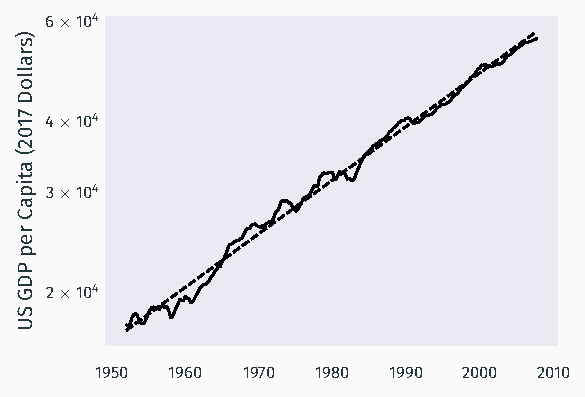
\includegraphics{figures/growth_effects.pdf}

    We're interested in understanding \alert{Business Cycles}
\end{frame}

\begin{frame}{Vector Autoregression (1/2)}
    Model a vector of outputs as an \alert{autoregressive process}

    \[
        Y_t = \sum_{\ell = 1}^p B_\ell Y_{t - \ell} + u_t
    \]
    Where:
    \begin{description}
        \item[$Y_t$] Vector of Outputs
        \item[$B_\ell$] Coefficient Matrix
        \item[$u_t$] Vector of Errors
    \end{description}
\end{frame}

\begin{frame}{Vector Autoregression (2/2)}
    \centering
    \begin{psmatrix}[colsep=1.5cm, rowsep=1cm]
    % nodes
    $\dots$ & $y_{1, t-3}$ & $y_{1, t-2}$ & $y_{1, t-1}$ & $y_{1, t}$ \\
    $\dots$ & $y_{2, t-3}$ & $y_{2, t-2}$ & $y_{2, t-1}$ & $y_{2, t}$ \\
    $\dots$ & $y_{3, t-3}$ & $y_{3, t-2}$ & $y_{3, t-1}$ & $y_{3, t}$

    % first column of arrows
    \ncline[nodesep=5pt]{->}{1,1}{1,2}
    \ncline[nodesep=5pt]{->}{1,1}{2,2}
    \ncline[nodesep=5pt]{->}{1,1}{3,2}
    \ncline[nodesep=5pt]{->}{2,1}{1,2}
    \ncline[nodesep=5pt]{->}{2,1}{2,2}
    \ncline[nodesep=5pt]{->}{2,1}{3,2}
    \ncline[nodesep=5pt]{->}{3,1}{1,2}
    \ncline[nodesep=5pt]{->}{3,1}{2,2}
    \ncline[nodesep=5pt]{->}{3,1}{3,2}

    % second column
    \ncline[nodesep=5pt]{->}{1,2}{1,3}
    \ncline[nodesep=5pt]{->}{1,2}{2,3}
    \ncline[nodesep=5pt]{->}{1,2}{3,3}
    \ncline[nodesep=5pt]{->}{2,2}{1,3}
    \ncline[nodesep=5pt]{->}{2,2}{2,3}
    \ncline[nodesep=5pt]{->}{2,2}{3,3}
    \ncline[nodesep=5pt]{->}{3,2}{1,3}
    \ncline[nodesep=5pt]{->}{3,2}{2,3}
    \ncline[nodesep=5pt]{->}{3,2}{3,3}

    % third column
    \ncline[nodesep=5pt]{->}{1,3}{1,4}
    \ncline[nodesep=5pt]{->}{1,3}{2,4}
    \ncline[nodesep=5pt]{->}{1,3}{3,4}
    \ncline[nodesep=5pt]{->}{2,3}{1,4}
    \ncline[nodesep=5pt]{->}{2,3}{2,4}
    \ncline[nodesep=5pt]{->}{2,3}{3,4}
    \ncline[nodesep=5pt]{->}{3,3}{1,4}
    \ncline[nodesep=5pt]{->}{3,3}{2,4}
    \ncline[nodesep=5pt]{->}{3,3}{3,4}

    % second column
    \ncline[nodesep=5pt]{->}{1,4}{1,5}
    \ncline[nodesep=5pt]{->}{1,4}{2,5}
    \ncline[nodesep=5pt]{->}{1,4}{3,5}
    \ncline[nodesep=5pt]{->}{2,4}{1,5}
    \ncline[nodesep=5pt]{->}{2,4}{2,5}
    \ncline[nodesep=5pt]{->}{2,4}{3,5}
    \ncline[nodesep=5pt]{->}{3,4}{1,5}
    \ncline[nodesep=5pt]{->}{3,4}{2,5}
    \ncline[nodesep=5pt]{->}{3,4}{3,5}
\end{psmatrix}

\end{frame}

\begin{frame}{Causal Inference (1/2)}
    Variance covariance matrix of $u_t$ is symmetric and dense

    VARs measure \alert{correlations}, not \alert{causation} {\scriptsize \parencite{nakamura2018identification}}

    Ex: Measured effect of interest rate on GDP could be:
    \begin{itemize}
        \item The interest rate responding to forecasts about GDP
        \item GDP actually responding to the interest rate
    \end{itemize} 
\end{frame}

\begin{frame}{Causal Inference (2/2)}
    A \alert{structural shock} is an exogenous shock to one of the variables in the model

    Could be caused by
    \begin{itemize}
        \item International events
        \item Other series movements
        \item ...
    \end{itemize}

    The effect of a structural shock to a variable is the \alert{causal effect} of changes in that variable
\end{frame}

\begin{frame}{Structural VAR (1/2)}
    Add a contemporaneous relationship to the VAR

    \[
        A_0 Y_t = \sum_{\ell = 1}^p A_\ell Y_{t - \ell} + \varepsilon_t
    \]
    Where:
    \begin{description}
        \item[$Y_t$] Vector of Outputs
        \item[$A_\ell$] Coefficient Matrix
        \item[$\varepsilon_t$] Vector of \alert{Structural} Errors (Var Cov Matrix $I_n$)
    \end{description}
\end{frame}

\begin{frame}{Structural VAR (2/2)}
    \centering
    \begin{psmatrix}[colsep=1.5cm, rowsep=1cm]
    % nodes
    $\dots$ & $y_{1, t-3}$ & $y_{1, t-2}$ & $y_{1, t-1}$ & $y_{1, t}$ \\
    $\dots$ & $y_{2, t-3}$ & $y_{2, t-2}$ & $y_{2, t-1}$ & $y_{2, t}$ \\
    $\dots$ & $y_{3, t-3}$ & $y_{3, t-2}$ & $y_{3, t-1}$ & $y_{3, t}$

    % first column of arrows
    \ncline[nodesep=5pt]{->}{1,1}{1,2}
    \ncline[nodesep=5pt]{->}{1,1}{2,2}
    \ncline[nodesep=5pt]{->}{1,1}{3,2}
    \ncline[nodesep=5pt]{->}{2,1}{1,2}
    \ncline[nodesep=5pt]{->}{2,1}{2,2}
    \ncline[nodesep=5pt]{->}{2,1}{3,2}
    \ncline[nodesep=5pt]{->}{3,1}{1,2}
    \ncline[nodesep=5pt]{->}{3,1}{2,2}
    \ncline[nodesep=5pt]{->}{3,1}{3,2}
    \ncline[nodesep=5pt]{->}{1,2}{2,2}
    \ncarc[nodesep=5pt,arcangle=-15]{->}{2,2}{3,2}
    \ncarc[nodesep=5pt,arcangle=-15]{->}{3,2}{2,2}

    % second column
    \ncline[nodesep=5pt]{->}{1,2}{1,3}
    \ncline[nodesep=5pt]{->}{1,2}{2,3}
    \ncline[nodesep=5pt]{->}{1,2}{3,3}
    \ncline[nodesep=5pt]{->}{2,2}{1,3}
    \ncline[nodesep=5pt]{->}{2,2}{2,3}
    \ncline[nodesep=5pt]{->}{2,2}{3,3}
    \ncline[nodesep=5pt]{->}{3,2}{1,3}
    \ncline[nodesep=5pt]{->}{3,2}{2,3}
    \ncline[nodesep=5pt]{->}{3,2}{3,3}
    \ncline[nodesep=5pt]{->}{1,3}{2,3}
    \ncarc[nodesep=5pt,arcangle=-15]{->}{2,3}{3,3}
    \ncarc[nodesep=5pt,arcangle=-15]{->}{3,3}{2,3}

    % third column
    \ncline[nodesep=5pt]{->}{1,3}{1,4}
    \ncline[nodesep=5pt]{->}{1,3}{2,4}
    \ncline[nodesep=5pt]{->}{1,3}{3,4}
    \ncline[nodesep=5pt]{->}{2,3}{1,4}
    \ncline[nodesep=5pt]{->}{2,3}{2,4}
    \ncline[nodesep=5pt]{->}{2,3}{3,4}
    \ncline[nodesep=5pt]{->}{3,3}{1,4}
    \ncline[nodesep=5pt]{->}{3,3}{2,4}
    \ncline[nodesep=5pt]{->}{3,3}{3,4}
    \ncline[nodesep=5pt]{->}{1,4}{2,4}
    \ncarc[nodesep=5pt,arcangle=-15]{->}{2,4}{3,4}
    \ncarc[nodesep=5pt,arcangle=-15]{->}{3,4}{2,4}

    % second column
    \ncline[nodesep=5pt]{->}{1,4}{1,5}
    \ncline[nodesep=5pt]{->}{1,4}{2,5}
    \ncline[nodesep=5pt]{->}{1,4}{3,5}
    \ncline[nodesep=5pt]{->}{2,4}{1,5}
    \ncline[nodesep=5pt]{->}{2,4}{2,5}
    \ncline[nodesep=5pt]{->}{2,4}{3,5}
    \ncline[nodesep=5pt]{->}{3,4}{1,5}
    \ncline[nodesep=5pt]{->}{3,4}{2,5}
    \ncline[nodesep=5pt]{->}{3,4}{3,5}
    \ncline[nodesep=5pt]{->}{1,5}{2,5}
    \ncarc[nodesep=5pt,arcangle=-15]{->}{2,5}{3,5}
    \ncarc[nodesep=5pt,arcangle=-15]{->}{3,5}{2,5}
\end{psmatrix}

\end{frame}

\begin{frame}{Our Model (1/2)}
    Estimate the order 4 VAR
    \[
        Y_t = \sum_{\ell = 1}^p B_\ell Y_{t - \ell} + u_t
    \]

    Where $Y_t$ is the vector of
    \begin{itemize}
        \item GDP ($x_t$)
        \item Government Spending ($g_t$)
        \item Government Revenue ($t_t$)
    \end{itemize}
\end{frame}

\begin{frame}{Our Model (2/2)}
    \begin{columns}
        \begin{column}{0.5\textwidth}
            Structural relationship:
            \begin{align*}
                u_t^x &= a_1 u_t^g + a_2 u_t^t + \varepsilon_t^x \\
                u_t^g &= b_1 u_t^x + b_2 \varepsilon_t^t + \varepsilon_t^g \\
                u_t^t &= c_1 u_t^x + c_2 \varepsilon_t^g + \varepsilon_t^t
            \end{align*}

            Assume:
            \begin{itemize}
                \item $b_1 = 0$, {\scriptsize Government response is delayed}
                \item $c_1 = 1.7$, {\scriptsize \textcite{lutz2010fiscal}}
                \item $b_2$ or $c_2 = 0$, {\scriptsize identification restriction}
            \end{itemize}
        \end{column}

        \begin{column}{0.5\textwidth}
            \centering
            \begin{psmatrix}[colsep=3cm, rowsep=1cm]
    % nodes
    $u_t^x$ & $\varepsilon_t^x$ \\
    $u_t^g$ & $\varepsilon_t^g$ \\
    $u_t^t$ & $\varepsilon_t^t$

    % first column of arrows
    \ncline[nodesep=5pt]{->}{2,1}{1,1}
    \ncarc[nodesep=5pt,arcangle=15]{->}{3,1}{1,1}
    \ncarc[nodesep=5pt,arcangle=-25,linewidth=1.5pt]{->}{1,1}{3,1}
    \ncline[nodesep=5pt]{->}{1,2}{1,1}
    \ncline[nodesep=5pt]{->}{2,2}{2,1}
    \ncline[nodesep=5pt]{->}{3,2}{3,1}
    \ncline[nodesep=5pt,linestyle=dashed,dash=3pt 2pt]{->}{2,2}{3,1}
    \ncline[nodesep=5pt,linestyle=dashed,dash=3pt 2pt]{->}{3,2}{2,1}
\end{psmatrix}


            {\scriptsize \parencite{blanchard2002empirical}}
        \end{column}
    \end{columns}
\end{frame}


\section{Data}

\begin{frame}{Data (1/2)}
    Get data on \alert{GDP}, \alert{Government Spending}, and \alert{Tax Revenues} from FRED between 1960 and 2007

    Then we:
    \begin{description}
        \item[Inflation Adjust] Divide by GDP deflator
        \item[Detrend] Get business cycle effects 
    \end{description}
\end{frame}

\begin{frame}{Data (2/2)}
    \centering
    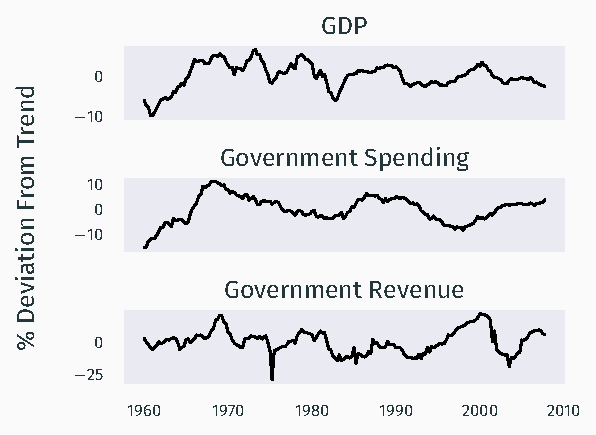
\includegraphics{figures/detrended_data.pdf}
\end{frame}


\section{Results}

\begin{frame}{IRFs} \label{frame:irfs}
    \centering
    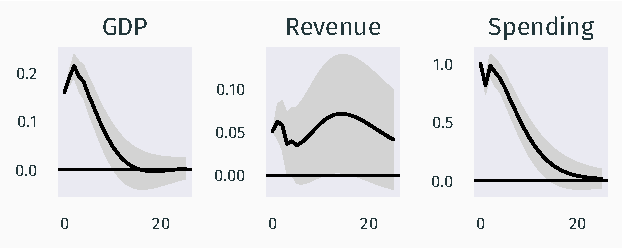
\includegraphics{figures/c20_irf.pdf}
    \hyperlink{frame:coefs}{\beamergotobutton{Coefficients}}
\end{frame}

\begin{frame}{Multiplier}
    Take the maximum increase in GDP following the structural shock

    Adjust for relative size of GDP and government spending

    Estimate multiplier is
    \begin{center}
        {\Large $1.035$}

        {\large $(0.115)$}
    \end{center}
\end{frame}

\begin{frame}{Robustness} \label{frame:robust}
    Results are robust to
    \begin{itemize}
        \item Setting $b_2 = 0$ \quad \hyperlink{frame:b20}{\beamergotobutton{Setting $b_2 = 0$}}
        \item Different responsiveness of revenue to GDP \quad \hyperlink{frame:c1}{\beamergotobutton{Changing $c_1$}}
        \item Using a different number of lags \quad \hyperlink{frame:order}{\beamergotobutton{VAR Order}}
        \item Allowing the effect to change over time \quad \hyperlink{frame:time}{\beamergotobutton{Time Trends}}
    \end{itemize}
\end{frame}


\section{Conclusion}

\begin{frame}{Conclusion}
    Using an SVAR, we estimated the fiscal multiplier for the US economy

    Found fiscal spending has approximately a 1-1 effect

    Limitations:
    \begin{itemize}
        \item Structural assumptions
        \item Simplistic linear detrending
        \item Revenue-side effects 
    \end{itemize}
\end{frame}


\begin{frame}[standout]
    Questions?
\end{frame}


\appendix


\begin{frame}{Coefficients} \label{frame:coefs}
    \centering
    \begin{tabular}{lccc}
        \toprule
        Parameter & $a_1$ & $a_2$ & $c_2$ \\
        \midrule
        Estimate & -0.182 & -0.150 & 0.040 \\
        \bottomrule
    \end{tabular}

    \hyperlink{frame:irfs}{\beamergotobutton{Back}}
\end{frame}


\begin{frame}{Setting $b_2 = 0$} \label{frame:b20}
    \centering
    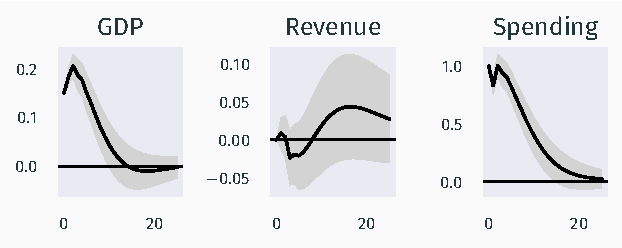
\includegraphics{figures/b20_irf.pdf}

    Multiplier: $0.990$ $(0.115)$

    \hyperlink{frame:robust}{\beamergotobutton{Back}}
\end{frame}

\begin{frame}{Changing $c_1$} \label{frame:c1}
    Follow \textcite{blanchard2002empirical}, set $c_1 = 2.08$

    \begin{center}
        \begin{tabular}{cccccc}
            \toprule
            \multicolumn{3}{c}{Parameter} & \multicolumn{3}{c}{Mutiplier} \\
            \cmidrule(lr){1-3} \cmidrule(lr){4-6}
            $a_1$ & $a_2$ & $c_2$ & Value & Std. Er. & Time \\
            \midrule
            -0.182 & -0.150 & 0.040 & 1.126 & 0.115 & 2 \\
            \bottomrule
        \end{tabular}

        \hyperlink{frame:robust}{\beamergotobutton{Back}}
    \end{center}
\end{frame}

\begin{frame}{Different VAR Orders} \label{frame:order}
    Estimate multiplier using VAR with order 1-24 (1 Quarter - 6 Years)

    \begin{center}
        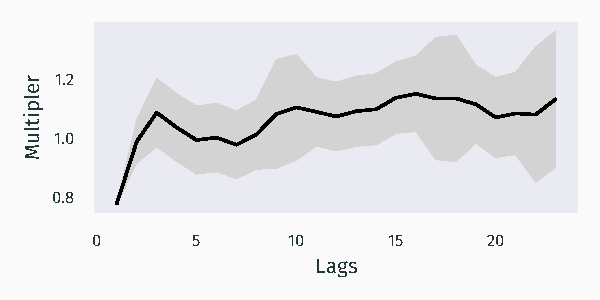
\includegraphics{figures/c20_lags.pdf}

        \hyperlink{frame:robust}{\beamergotobutton{Back}}
    \end{center}
\end{frame}

\begin{frame}{Time Trends} \label{frame:time}
    Estimate multiplier within 10 year rolling windows

    \begin{center}
        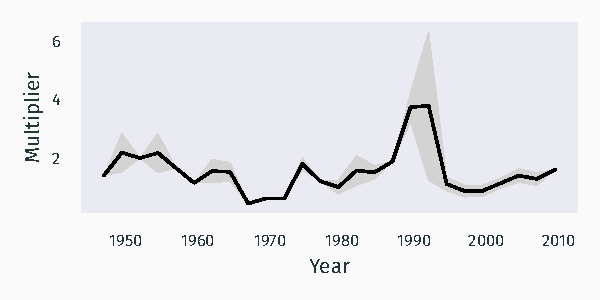
\includegraphics{figures/c20_ts.pdf}

        \hyperlink{frame:robust}{\beamergotobutton{Back}}
    \end{center}
\end{frame}

\begin{frame}[allowframebreaks]{References}
    \printbibliography[heading=none]
\end{frame}


\end{document}
